
\section{Điều chế và Giải điều chế PSK (Phase Shift Keying)}
\subsection{Giới thiệu về PSK}
PSK là sơ đồ điều chế kỹ thuật số truyền dữ liệu bằng cách thay đổi hoặc điều chế
pha của tín hiệu tham chiếu (sóng mang). PSK sử dụng một số giai đoạn hữu hạn, mỗi
giai đoạn được gán một mẫu chữ số nhị phân duy nhất. Thông thường, mỗi pha mã hóa
một số bit bằng nhau. Mỗi mẫu bit định dạng biểu tượng được biểu thị bằng pha cụ thể. \\
Trong hệ thống điều chế BPSK, tín hiệu băng tần gốc được gắn vào sóng mang bằng
cách thay đổi pha của sóng mang tùy thuộc vào tín hiệu băng gốc. \\
Giả sử có sóng mang được biểu diễn: \\
 $ x_{0}(t) = A.\sin(\omega_{0} + \varphi) $\\
Biểu thức tín hiệu gốc: S(t) là tín hiệu nhị phân (0,1) hay là chuỗi NRZ. \\ 
Do đó ta có: \\ 
- Khi $ s(t) = 0: P(t) = A.sin(\omega_{0}) $ \\
- Khi $ s(t) = 0: P(t) = A.sin(\omega_{0} + \pi) $ \\ 

Đối với khóa dịch pha PSK, thông tin chứa trong pha tức thời của sóng mang điều chế.
Thường thì pha này được ấn định và so sánh tương thích với sóng mang của pha đã biết
- PSK kết hợp. Kiểu điều chế BPSK này còn được gọi là điều chế khóa đảo pha PRK
(Phase Reversal Keying). Hình 7.7, trình bày bộ phát PRK, dạng sóng tín hiệu và phổ.
\begin{center}
     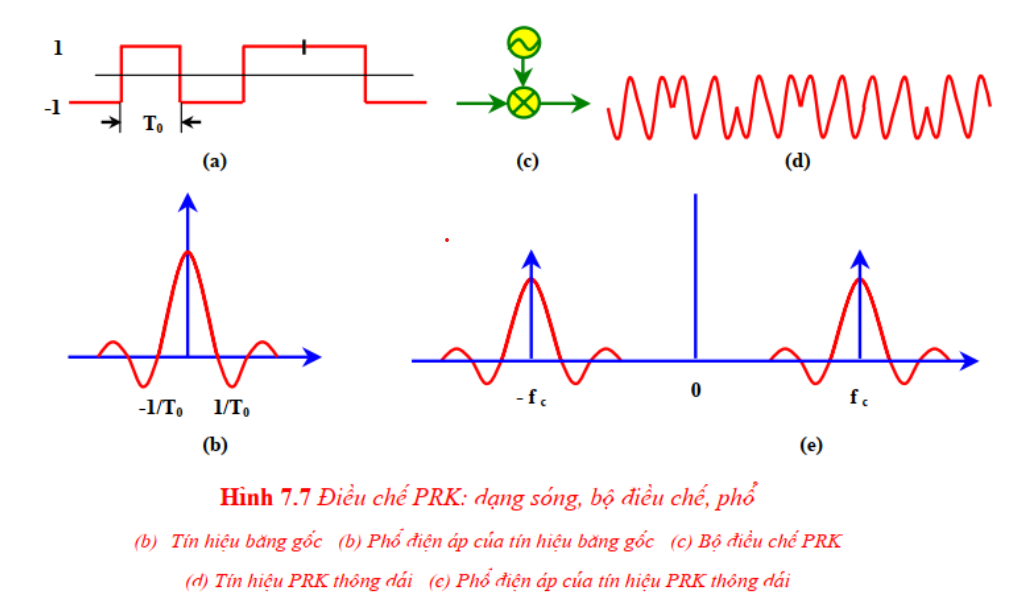
\includegraphics[scale=.5]{Img/dieuchepho.png}
\end{center}
\subsection{Nguyên tắc khóa dịch pha nhị phân}
Nguyên tắc : Các tín hiệu nhị phân tác dụng lên sóng mang làm thay đổi pha của
sóng mang. Cụ thể là: \\ 
• Bit 1: pha của sóng mang là 0. \\ 
• Bit 0: pha của sóng mang là $ 180^{o}.$\\  
Bảng chân lý của tín hiệu điều chế BPSK:
\begin{center}
     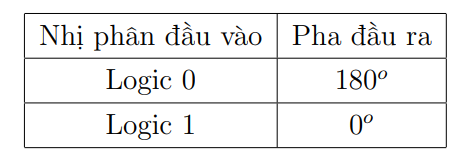
\includegraphics[scale=.5]{Img/bangchanlyPSK.png}
\end{center}
Có thể thấy rõ hơn trong cách biểu diễn trên đồ thị thời gian và trạng thái của tín
hiệu BPSK.
\begin{center}
     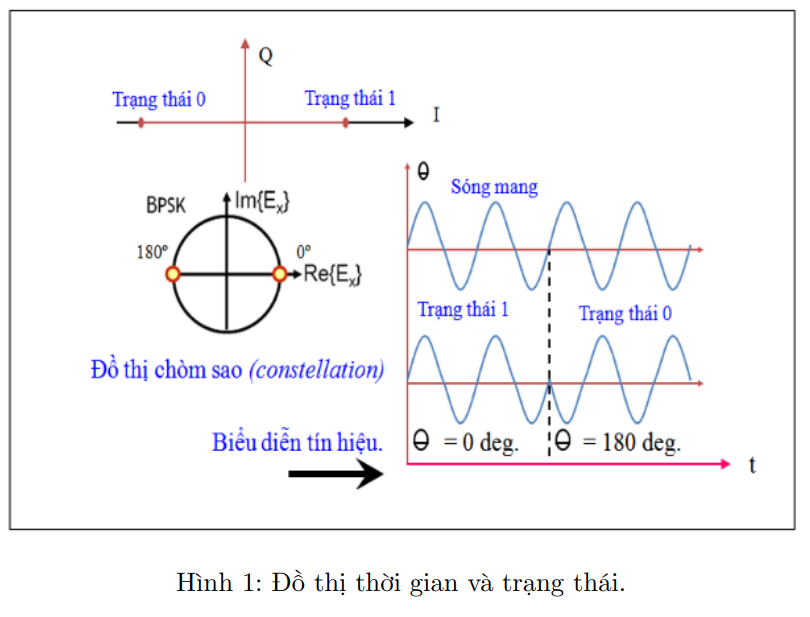
\includegraphics[scale=.7]{Img/bangtrangthai.png}
\end{center}
\subsection{Điều chế PSK}
\begin{center}
     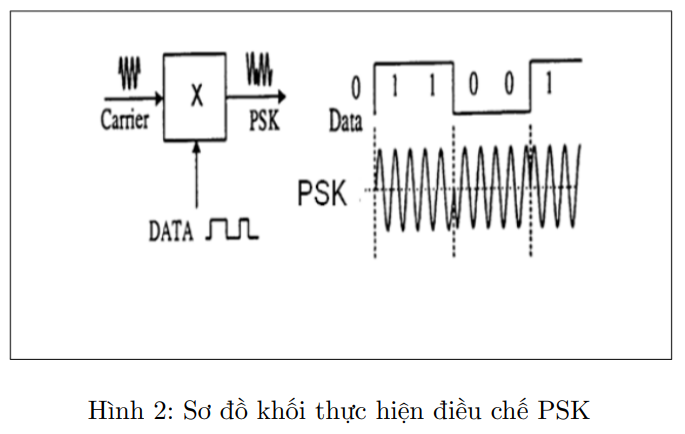
\includegraphics[scale=.7]{Img/sododieuchePSK.png}
\end{center}
Phương pháp điều chế 2-PSK hay BPSK (Binary PSK) hay điều chế ngược pha (Phase
Reversal Keying) được giới thiệu ở hình trên. \\ Sơ đồ tạo tín hiệu BPSK dạng sin với hai giá trị pha tùy thuộc vào giá trị Data: \\ 
- Khi data bit = 1, tín hiệu BPSK cùng pha với sóng mang \\ 
- Khi data bit = 0, tín hiệu BPSK ngược pha ($180^{o}$) với sóng mang. \\ 
\begin{center}
     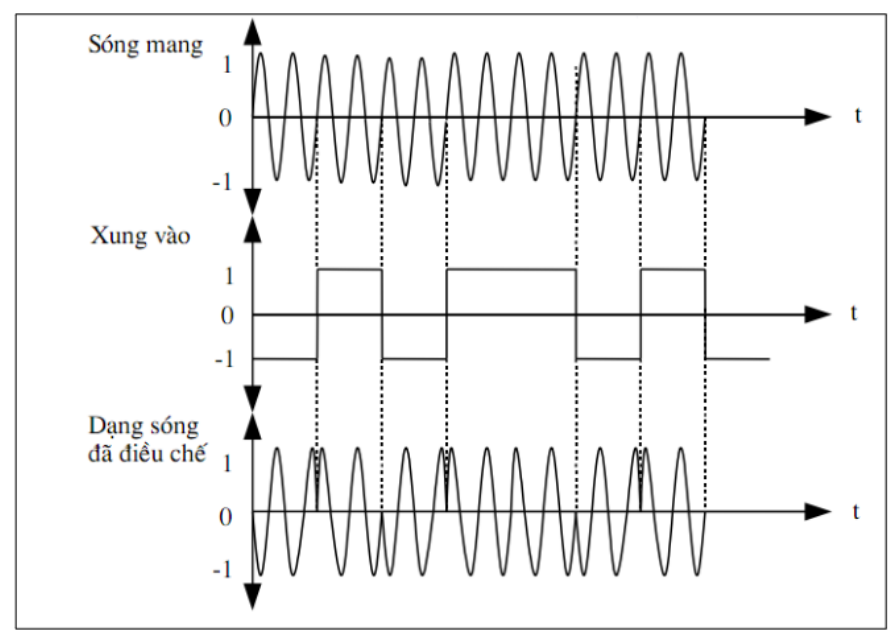
\includegraphics[scale=.5]{Img/quanhethoigiandieuche.png} \\ 
     Hình 3: Quan hệ pha/thời gian \\  ở đầu ra bộ điều chế PSK theo tín hiệu vào
\end{center}  \\
\newpage
\textbf{Mô hình điều chế PSk}
\begin{center}
    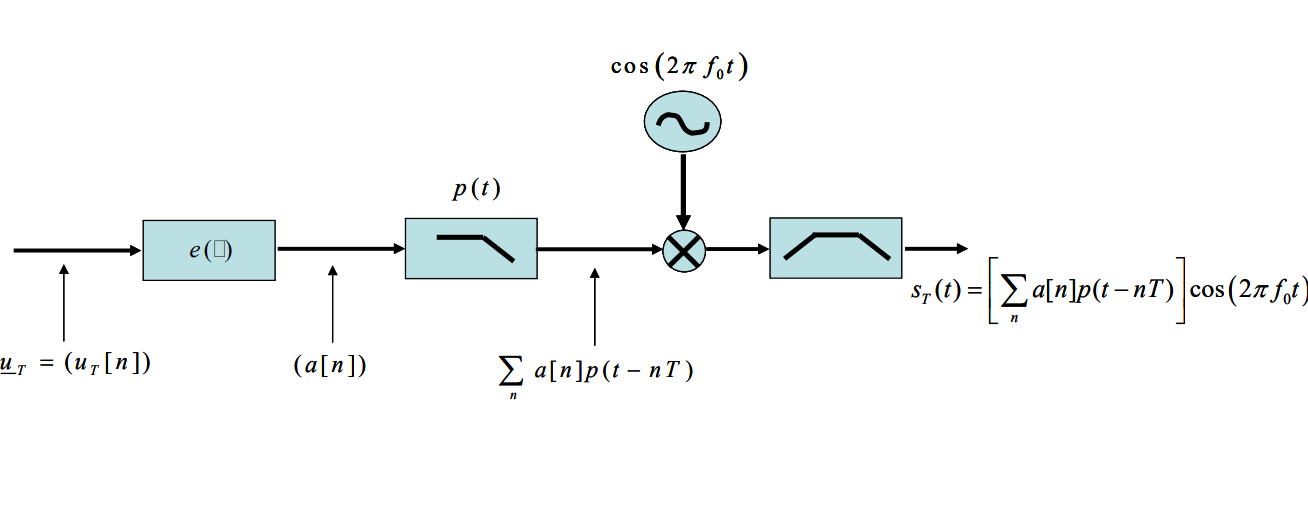
\includegraphics[scale=.6]{Img/bieudoASK.png}
\end{center}
\begin{center}
    \textbf{Mô hình điều chế PSK}
\end{center}

\newpage
\subsection{Mã nguồn điều chế tín hiệu PSK sử dụng ngôn ngữ Python, trình bày Jupyter Notebook }
\\ 
\textbf{ - Thêm thư viện} \\
import random \\ 
import numpy as np \\
import matplotlib.pyplot as plt \\ 
from scipy.signal import butter, filtfilt \\ 
\textbf{hàm tạo mảng bit ngẫu nhiên} \\ 
\begin{lstlisting}
def random_bits_array(n):   
    return [random.randint(0, 1) for _ in range(n)] 
\end{lstlisting}
\textbf{Hàm tạo tín hiệu xung vuông và xung vuông đảo ngược}
\begin{lstlisting}
def message_signal(m,T):                         
    t = np.arange(0, T, T/100)             
    message = []                           
    not_message = []
    for i in range(len(m)): 
        if m[i] == 1:                     
            m_s = np.ones(len(t))          
            invm_s = np.zeros(len(t))
        else:
            m_s = np.zeros(len(t))         
            invm_s = np.ones(len(t))       
        message.extend(m_s)                 
        not_message.extend(invm_s)         
    return message , not_message    
    
\end{lstlisting}
\textbf{khai báo}
\begin{lstlisting}
N = 8    
T = 1        
Tb = 1*N      
t = np.arange(0, Tb, Tb/800)  
m = random_bits_array(N) 
fc = 2                                         
songmang = np.sqrt(2/Tb) * np.sin(2 * np.pi * fc * t)  
\end{lstlisting}
\textbf{Vẽ sóng mang}
\begin{lstlisting}
fig, ax = plt.subplots(1, 1, figsize=(15, 2))   
fig.subplots_adjust(hspace=0.5)                 
ax.plot(t, c)                                  
ax.set_title('Tin hieu song mang')           
ax.set_xlabel('t --->')
ax.set_ylabel('c1(t) ---> ')
\end{lstlisting}
\begin{center}
     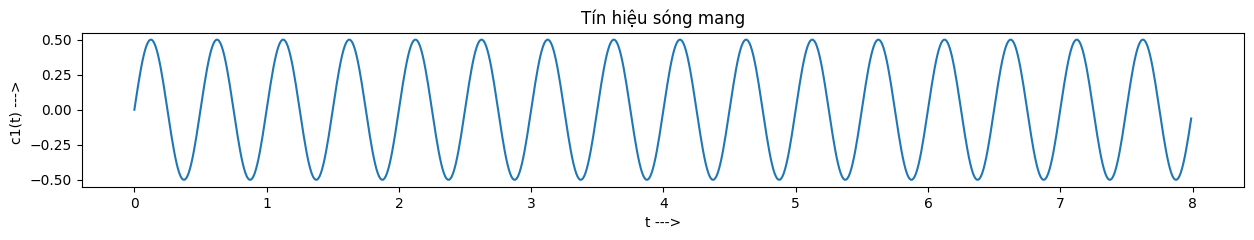
\includegraphics[scale=.5]{Img/tinhieusongmang.png}
\end{center}

\textbf{Vẽ chuỗi nhị phân và xung vuông tương ứng}
\begin{lstlisting}
fig, ax = plt.subplots(2, 1, figsize=(15, 5))               
fig.subplots_adjust(hspace=0.5)                           
ax[0].stem(m)                                          
ax[0].set_title('Chuoi nhi phan sinh ngau nhien')
ax[0].set_xlabel('n -->')
ax[0].set_ylabel('b(n) --->')
message , not_message = message_signal(m,T)                
print(len(message), len(not_message))
ax[1].plot(t,message, 'r')                                 
ax[1].set_title('Tin hieu xung vuong')
ax[1].set_xlabel('t --->')
ax[1].set_ylabel('c1(t) --->')
\end{lstlisting}
\begin{center}
     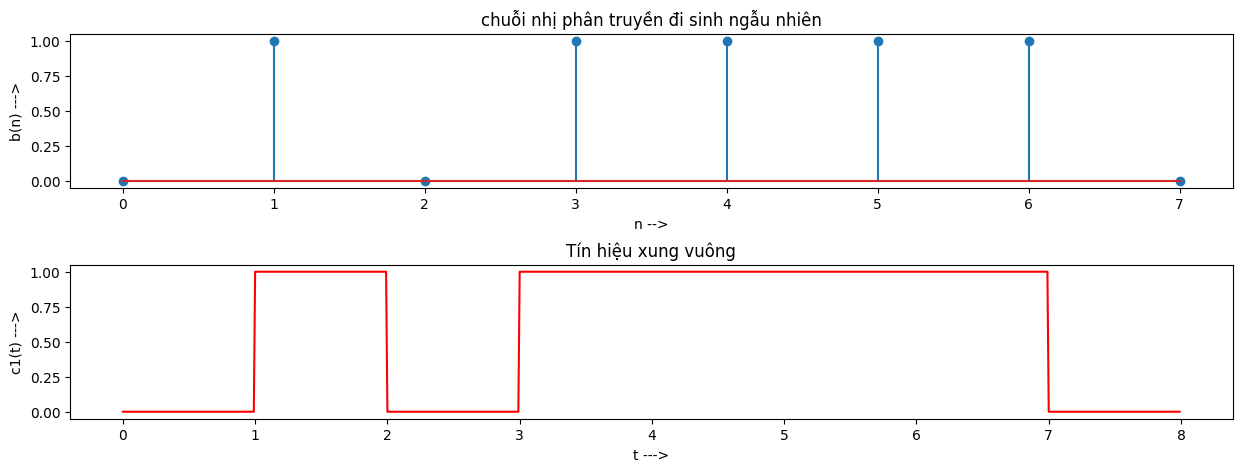
\includegraphics[scale=.5]{Img/vechuoinhiphantuognung.png}
\end{center}
\textbf{Điều chế PSK}
\begin{lstlisting}
def modulation(message_signal,not_message_signal):              
    return message_signal*songmang
            - not_message_signal*songmang  
psk = modulation(message,not_message)                              
\end{lstlisting}
\textbf{Tín hiệu PSK sau khi điều chế}
\begin{lstlisting}
fig, ax = plt.subplots(1, 1, figsize=(15, 2))    
ax.figsize=(15, 5)
ax.plot(t,psk, 'b')
ax.set_title('PSK signal')
ax.set_xlabel('t---->')
ax.set_ylabel('Gia tri')
\end{lstlisting}
\begin{center}
     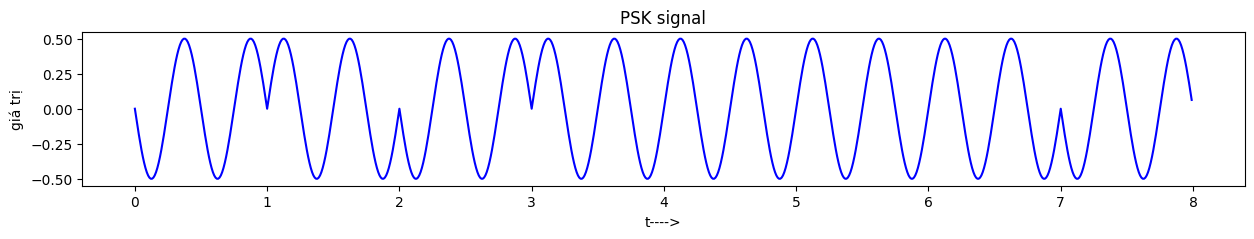
\includegraphics[scale=.5]{Img/tinhieuPSKsaukhidieuche.png}
\end{center}
\subsection{Giải điều chế PSK}
\textbf{Bộ giải điều chế BPSK bao gồm:} \\
- Sơ đồ lấy bình phương để chuyển các tín hiệu khác pha về cùng 1 pha \\ 
- Vòng giữ pha PLL phát lại nhịp với tần số gấp đôi tần số sóng mang \\ 
- Bộ chia pha $\Delta\phi$ để hiệu chỉnh pha \\ 
- Bộ chia hai để đưa tần số tín hiệu tái lập về bằng tần số sóng mang \\ 
- Bộ nhân tín hiệu thực hiện nhân sóng điều chế PSK với sóng mang tái lập \\ 
Giả sử tần số sóng mang là fc, $\omega$ c = 2$\pi$fc, ta có hai trường hợp: \\ 
Khi tín hiệu PSK là $+\sin(\omega_{c}t)$ ứng với Data bit = 1, sóng mang tái lập là $\sin(\omega_{c}t)$, sơ đồ nhân sẽ cho tín hiệu: \\
$\sin(\omega_{c}t).\sin(\omega_{c}t)) = \sin(\omega_{c}t)^{2}$
$ = \frac{1}{2}.(1 - \cos(2\omega_{c}t)) = \frac{1}{2} - \frac{1}{2} \cos(2.\omega_{c}t)$
Trong biểu thức trên, thành phần thứ hai là xoay chiều, có tần số gấp đôi tần số sóng mang. Khi sử dụng bộ lọc thông thấp với tần số cắt bằng tần số sóng mang, ta có thể khử bỏ thành phần xoay chiều và thế dương của thành phần một chiều thứ nhất được giữ lại sẽ biểu diễn trạng thái "1" của bit Data.

Khi tín hiệu PSK là $-\sin(\omega_{c}t)$ ứng với Data bit = 0,sơ đồ nhân sẽ cho tín hiệu \\
$-\sin(\omega_{c}t).\sin(\omega_{c}t)) = -\sin(\omega_{c}t)^{2}$
$ = -\frac{1}{2}.(1 - \cos(2\omega_{c}t)) = -\frac{1}{2} + \frac{1}{2} \cos(2.\omega_{c}t)$
Trong biểu thức trên, thành phần thứ hai là xoay chiều, có tần số gấp đôi tần số sóng mang. \textbf{Khi sử dụng bộ lọc thông thấp với tần số cắt bằng tần số sóng mang, ta có thể khử bỏ thành phần xoay chiều} và thế âm của thành phần một chiều thứ nhất được giữ lại sẽ biểu diễn trạng thái "0" của bit Data.
\subsection{Mã nguồn giải điều chế tín hiệu PSK sử dụng ngôn ngữ Python,
trình bày Jupyter Notebook}
\textbf{Hàm giải mã tín hiệu}
# Nếu tín hiệu mẫu trùng với sóng sin được sử dụng, thì tổng của tích sóng sẽ lớn, 
# còn nếu tín hiệu mẫu không trùng với sóng sin được sử dụng, tổng của tích sóng sẽ nhỏ.
# Để tính tổng này, chúng ta dùng vòng lặp để chạy qua mỗi giá trị của N, 
# tính tổng với khoảng tín hiệu tương ứng, rồi cập nhật giá trị start và end cho lần chạy tiếp theo của vòng lặp.
\begin{lstlisting}
    def demodulation(filtered_signal,N):                                # giải mã tín hiệu nhận được
    start = 0
    end = 100
    demod = np.zeros(N)
    for i in range(N):
        x = np.sum(songmang[start:end] 
                * filtered_signal[start:end])
        if x > 0:
            demod[i] = 1
        else:
            demod[i] = 0
        start += 100
        end += 100
    return demod
\end{lstlisting}
\textbf{Vẽ tín hiệu sau khi điều chế }
\begin{center}
     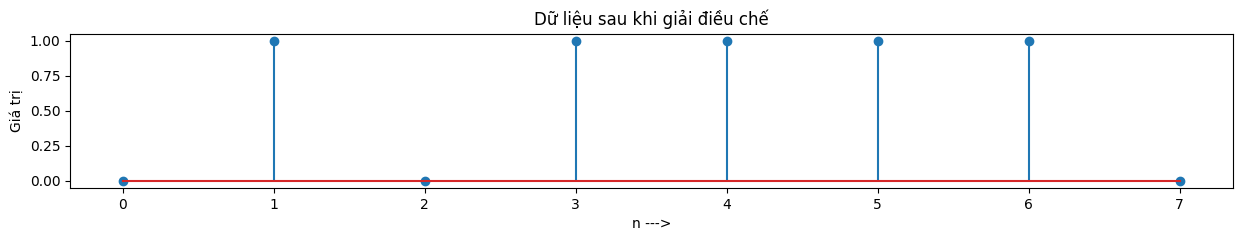
\includegraphics[scale=.5]{Img/dulieusaudieuche.png}
\end{center}
\newpage
\section{ Điều tra điều chế/giải điều chế PSK dưới tác động của nhiễu Gaussian }
Nhiễu Gaussian là một tín hiệu ngẫu nhiên có mật độ phân bố công suất phẳng nghĩa làtín hiệu nhiễu có công suất bằng nhau trong toàn khoảng băng thông. Tín hiệu này có tên là nhiễu trắng vì nó có tính chất tương tự với ánh sáng trắng. Chúng ta không thể tạo ra nhiễu trắng theo đúng lý thuyết vì theo định nghĩa của nó, nhiễu trắng có mật độ phổ công suất phân bố trong khoảng tần vô hạn và do vậy nó cũng phải có công suất vô hạn. Tuy nhiên, trong thực tế, chúng ta chỉ cần tạo ra nhiễu trắng trong khoảng băng tần của hệ thống chúng ta đang xem xét. \\ 
Với khóa dịch pha nhị phân (PSK), các bit nhị phân 1 và 0 có thể được biểu thị
bằng các mức năng lượng tương ứng : $+\sqrt{E_{b} $ và $-\sqrt{E_{b} $.
\begin{center}
     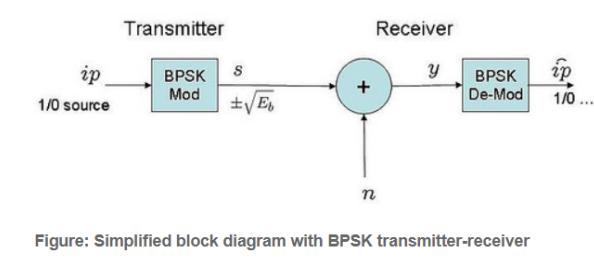
\includegraphics[scale=.5]{Img/Gausodo1.png}
\end{center}
\subsection{Thêm nhiễu Gaussian vào dạng sóng truyền đi}
\textbf{a) Khi sóng truyền có dạng} r(t) = s(t) + n(t), 0 ≤ t ≤ Tb.
\begin{center}
     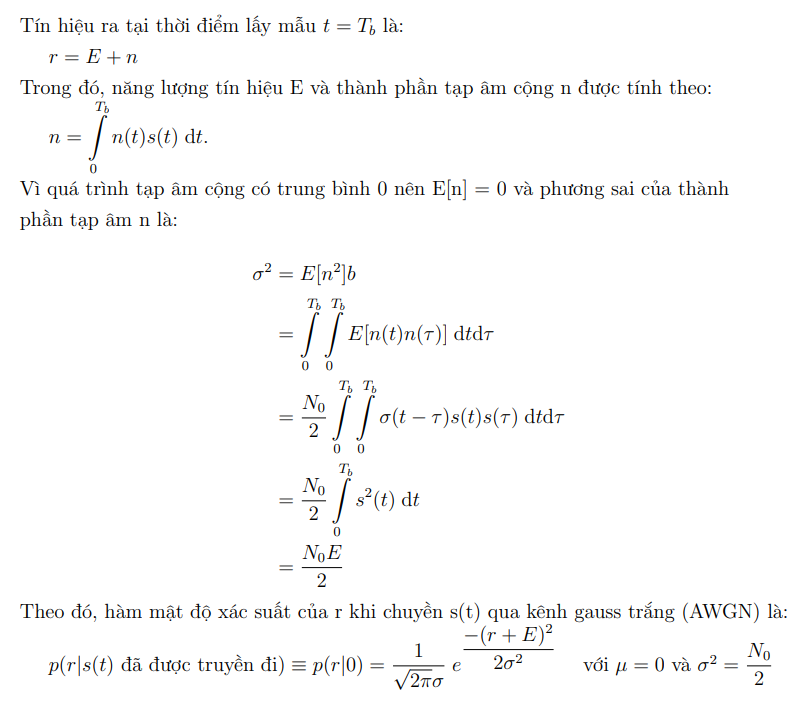
\includegraphics[scale=.6]{Img/tichphannangluong.png}
\end{center}
\begin{center}
     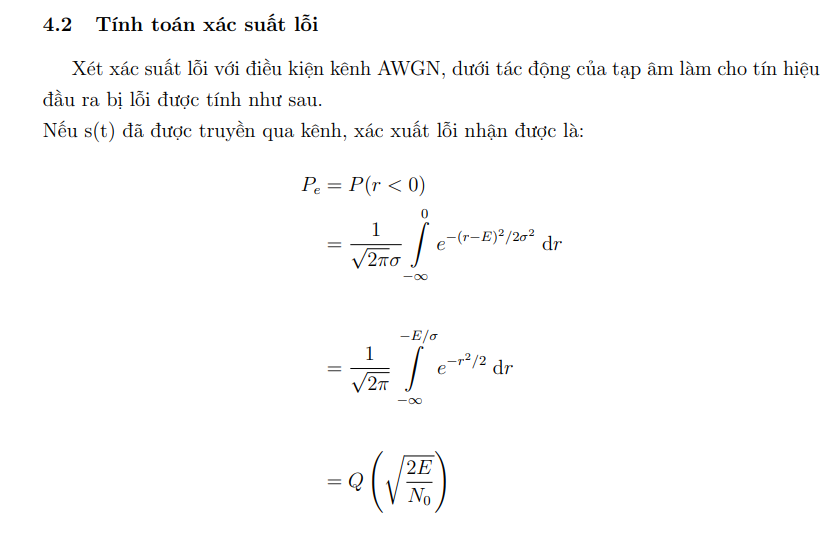
\includegraphics[scale=.7]{Img/tinhtoanxacsuatloi.png}
\end{center}
\newpage
\subsection{Mã nguồn điều chế tín hiệu/ giải điều chế có sự can thiệp bởi nhiễu Gaussian PSK sử dụng ngôn ngữ Python, trình bày Jupyter Notebook }
\textbf{Thêm nhiễu Gaussian với phương sai N0/2, giá trị trung bình = 0}
\begin{lstlisting}
N0 = 2
noise = np.random.normal(0, np.sqrt(N0/2), psk.shape)          
psk_noisy = psk + noise #r(t) = s(t) + n(t)                    
\end{lstlisting}
\textbf{Vẽ tín hiệu khi đã thêm nhiễu nhiệt}
\begin{lstlisting}
fig, ax = plt.subplots(1, 1, figsize=(15, 5))
ax.plot(t, psk_noisy, 'r')
ax.set_title('Tin hieu PSK, nhieu Gaussian')
ax.set_xlabel('t---->')
ax.set_ylabel('Gia tri')
plt.show()
\end{lstlisting}
\begin{center}
     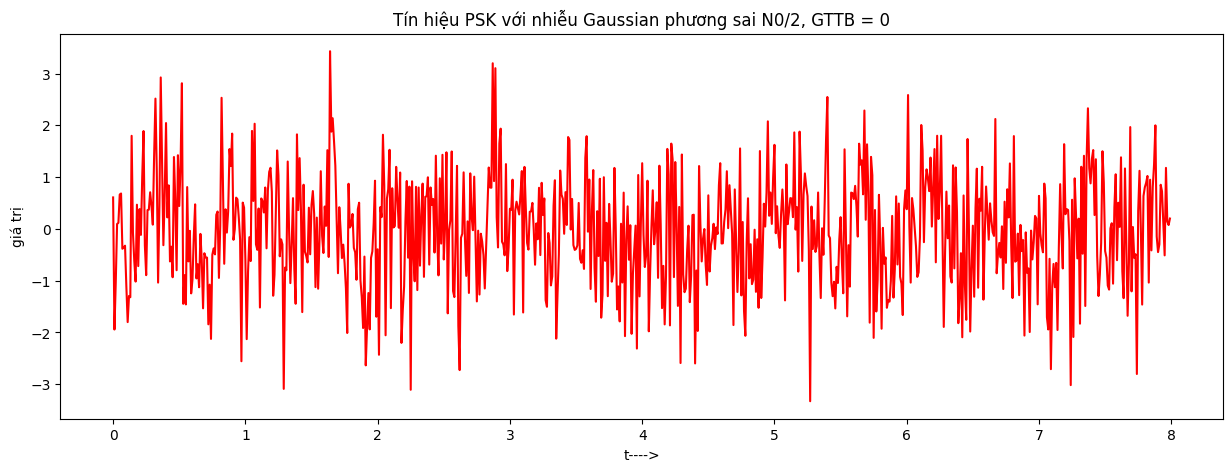
\includegraphics[scale=.5]{Img/venhieu.png}
\end{center}
\newpage
\textbf{Giải nhiễm Gaussian}
\begin{lstlisting}
def gaussian_noise_cancellation(signal, 
                        cutoff=0.05, order=5):        
    b, a = butter(order, cutoff, btype='low', analog=False)            
    filtered_signal = filtfilt(b, a, signal)                           
    return filtered_signal                                  
\end{lstlisting}
\textbf{Vẽ tín hiệu sau khi giải nhiễu}
\begin{center}
     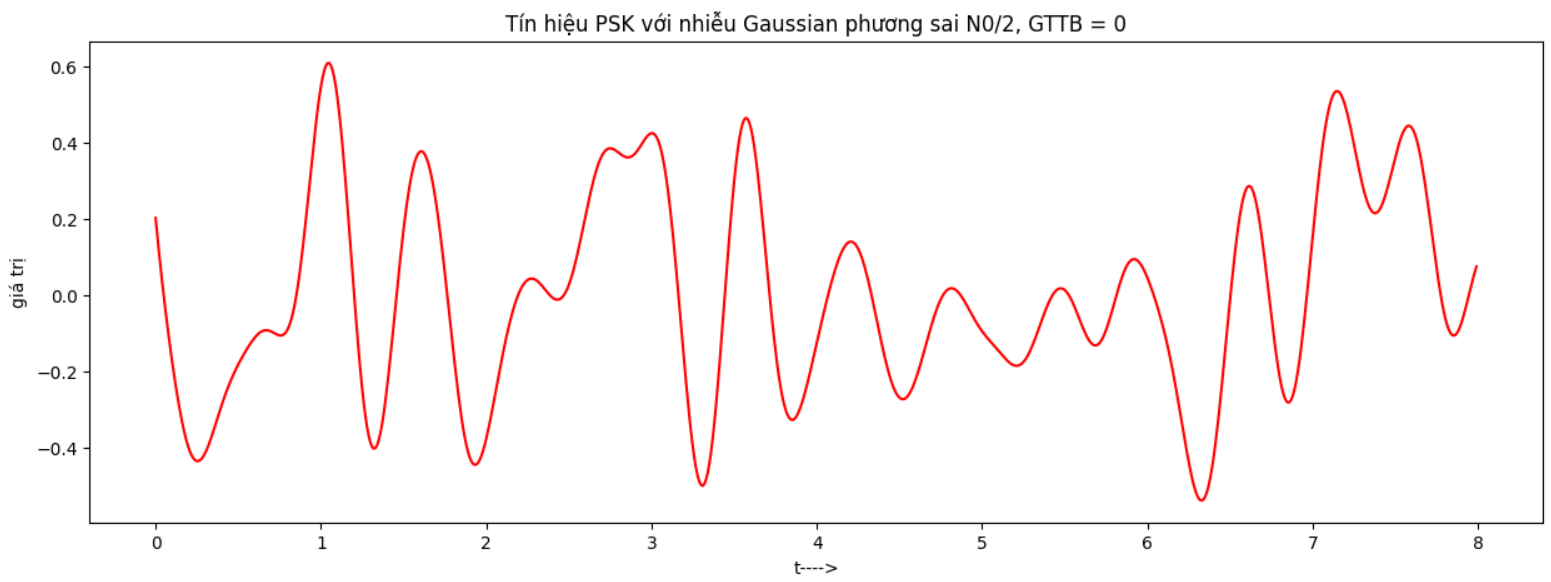
\includegraphics[scale=.5]{Img/giainhieu.png}
\end{center}
\newpage
\section{Tính xác suất lỗi bit của kênh Gaussian PSK}
\subsection{Xác suất lỗi bit theo lí thuyết}
\begin{center}
     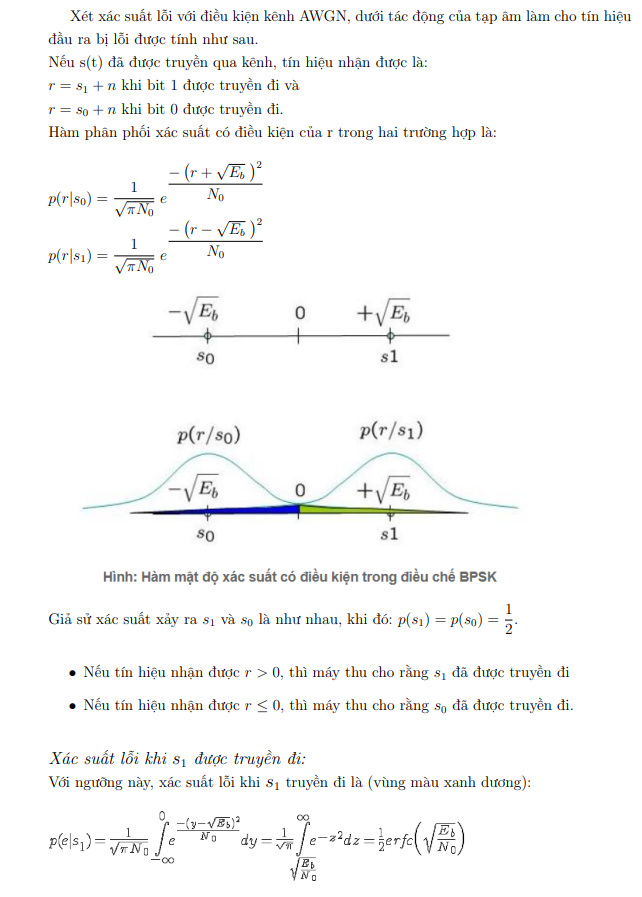
\includegraphics[scale=1]{Img/tinhxacsuatloibitkenhGau.png}
\end{center}
\newpage
\begin{center}
     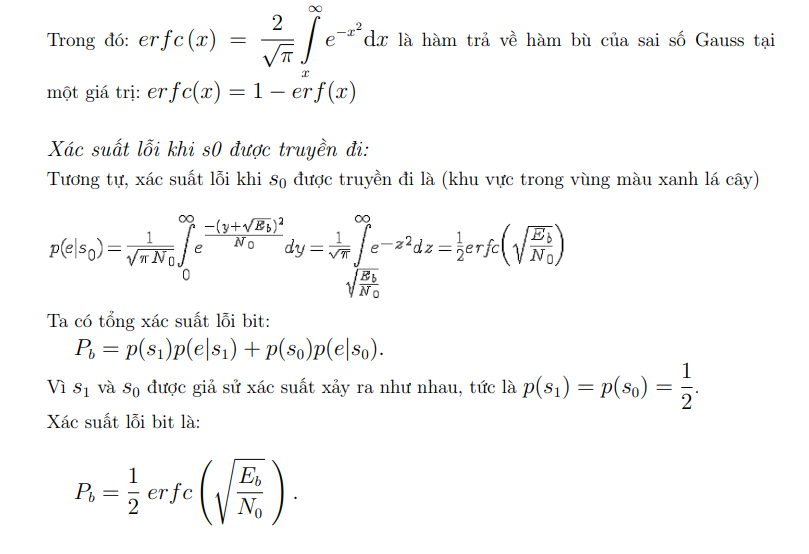
\includegraphics[scale=.8]{Img/tinhxacsuatloibitkenhGau2.png}
\end{center}
\newpage
\subsection{Mã nguồn tính xác suất lỗi bit}
\begin{lstlisting}
    def calculate_bit_error_rate(bitBanDau, bitNhanDuoc):
    num_errors = 0
    for i in range(len(bitBanDau)):
        if bitBanDau[i] != bitNhanDuoc[i]:
            num_errors += 1
    ber = num_errors / len(bitBanDau)
    return ber
    bitBanDau = m
    bitNhanDuoc = demod
    ber = calculate_bit_error_rate(bitBanDau, bitNhanDuoc)
    print("Xác xuất lỗi bit: {:.2f}%".format(ber * 100))
\end{lstlisting}



